\documentclass[11pt, letterpaper, onecolumn]{article}
\usepackage{cite}
\usepackage{amsmath}
\usepackage{algorithm}
\usepackage{algorithmic}
\usepackage{graphicx}
\usepackage{subcaption}
\usepackage{csvsimple}

\title{\textbf{Metaheuristics for the MDMKP}}


\begin{document}
\maketitle

\section{Goals}

Metaheuristics commonly have a wide array of parameters that must be tuned in order to
obtain good performace. This task is often time consuming, and can lead to brittle systems
ill-equiped to handle changing problems. Instead, we focus solely on metaheuristics that
do not require any parameter tuning. These methods often have the added effect of being
simple and easy to implement, while still giving competitive results.

\section{Algorithms Used}

\subsection{Jaya}

Jaya is a metaheuristic proposed by Dr.~Rao of the Sardar Vallabhbhai National
Institute of Technology%\cite{jaya}
. It was originally developed to work on continous
problems, but has been modified to work on binary problems.

Jaya creates a new solution by moving an existing solution towards the best solution found, while simultaneously moving it away from the worst solution found. In the continous space, each movement vector is scaled by some continous value between zero and one. However, as the MDMKP is a binary formulation, there are no fractional movements. Instead, each bit is scaled either 0\% or 100\% of it's distance vector. 

A strict conversion of the Jaya algorithm would require that the 0\% solution is selected over the 100\% solution according to two randomly chosen probabilites, one for the best solution, and one for the worst. However, testing has shown that a strategy that uniformly selects scaling factors outperforms weighted selection. This uniform selection strategy is formally defined as follows: 

 Given a population $X$, define $best$ as the best performing solution, and $worst$ as the worst performing solution. $r$ is the random function, and uniformly selects an element from the set. For every solution $S$ in the population, construct a modified solution according to the following transformation applied to every bit $i$ in $S$:
\begin{equation} S_i' = S_i + r(\{0, 1\})*(best_i - S_i) - r(\{0, 1\})*(worst_i - S_i) > 0 \end{equation}

For the faithful but worse performing method, the following transformation is used, where $bs$ is the scaling factor from 0 to 1 for the best solution, and $ws$ is the worst solution scaling factor: 
\begin{equation}\label{jayav2} S_i' = S_i + (r([0,1])<bs)*(best_i - S_i) - (r([0, 1])<ws)*(worst_i - S_i) > 0 \end{equation}

Jaya instances using equation \ref{jayav2} are refered to as "jaya\_v2" in this implementation, while the uniform method is just "jaya". 

If the new solution generated by the Jaya transformation is valid and performs better than the old solution, replace it in the population. One iteration of Jaya will attempt this transformation for every solution in the population. 

In this implementation, a modification of Jaya is used. Instead of using the best and worst solution every time, parameters $m$ and $n$ are generated, such that the best solution is selected from $random(sorted\_population[start:m])$, and the worst solution is selected from $random(sorted\_population[end-n:end])$. This introduces two parameters to the metaheuristic, a violation of the goals. However, higher $m$ and $n$ values improve performance. 

\subsection{TLBO}

Teaching-Learning Based Optimization is another metaheuristic developed by Dr.~Rao for continous problems %\cite{TLBO}
. It is a two phase algorithm: the Teaching phase, and the Learning phase.

\subsubsection{TBO}

The first phase, Teaching Based Optimization, constructs new solutions by moving a given solution along the distance vector found by moving from the mean solution to the best solution. The vector is sometimes doubled. Once again, partial movements are impossible, so a 0\% or 100\% strategy is applied to each individual bit. Formally, it is defined as follows: For every bit index $i$ in a solution $S$, update a new solution according to: 
\begin{equation}
S_i' = \Big(S_i + r(\{0, 1\})*\big(best_i - r(\{1, 2\})*average_i\big)\Big) > 0
\end{equation}
where $best$ is the best scoring solution in the population, and $average$ is the average of all solutions in the population. 

There are two different methods for calculating the average value. The first is to order the population by objective function values, and then use the middle solution as the median average. However, this has a different intent than the continous method: instead of acting as the centerpoint of the population, it is an effectively randomly chosen midtier solution. 

Instead, the mean is calculated as it would be in the continous space. This will results in a vector of numbers between 0 and 1. This can be converted to a discrete representation by treating the values as a likelihood chance of being turned on, like so: 
\begin{equation}\label{tbouniform}
S_i' = \Big(S_i + r(\{0, 1\})*\big(best_i - r(\{1, 2\})*(r([0, 1]) < average_i)\big)\Big) > 0
\end{equation}
Notice that the random function $r$ was given a continous range from 0 to 1, not a discrete set. This probability method has been shown to give better results than the median method in testing. 

Equation \ref{tbouniform} uses a uniform selection strategy, much like the uniform Jaya variant. A weighted TBO variant has also been implemented, and is reffered to as``TBO\_v2" in this implementation. With a weight $w$ uniformly selected from 0 to 1, the weighted perturbation is defined as follows: 
\begin{equation}\label{tbouniform}
S_i' = \Big(S_i + (r([0,1])<w)*\big(best_i - r(\{1, 2\})*(r([0, 1]) < average_i)\big)\Big) > 0
\end{equation}

The TBO transform is used in the same way as the jaya transform: apply to every solution in the population, and replace the solutions if the new solutions have better objective function scores.

Dr.~Rao originally specified that, much like Jaya, only the absolutely best solution is used. But one again, performance is improved by randomly selecting a solution from some $n$ of top solutions. 

Similarly, the mean could be calculated from a subset of the population, instead of the whole, in order to increase the variety of generated solutions. However, this would be computationally expensive, and TBO already produces some of the most diverse populations of any metaheuristic implemented here. 

\paragraph{CBO}

In the same way solutions are moved according to the vector from the mean to a selected good solution, they can be moved according to the vector from a selected bad solution to the mean. This is referred to as Clown Based Optimation, and is otherwise implemented identically to TBO. 

\subsubsection{LBO}

The second phase of TLBO, Learning Based Optimization, acts by selecting two solutions, and moving the worse performing solution some distance along the vector between them\footnote{It is worth noting that the vector from the better to the worse solution contains all the same points as the vector from the worse to the better---the only difference is what solution is replaced, if the new solution yields an improved score.}. In the binary space, the vector between points becomes a set of shortest paths from one solution to another, from which a new solution is selected.  If the new solution has a better score than the worse performing solution, it is replaced. Solutions cannot be the same. In this implementation, a single instance of LBO is guaranteed to act on every solution at least once, like so:

\begin{algorithm}
\caption{Learning Based Optimization}
\begin{algorithmic}
\FOR{$sol_1 \in X$}
\STATE $sol_2 = rand(X)$
\WHILE{$sol_1 = sol_2$} 
\STATE $sol_2 = rand(X)$
\ENDWHILE
\STATE{$student, teacher = sort(sol_1, sol_2)$}
\STATE{$new\_student = copy(student)$}
\FOR{$i \in 0..length(student)$}
\STATE $new\_student_i \mathrel{{+}{=}} rand(\{0,1\}) * (teacher_i - student_i)$
\ENDFOR
\IF{$score(new\_student) > score(student)$}
\STATE{$X_{student} = new\_student$}
\ENDIF
\ENDFOR
\end{algorithmic}
\end{algorithm}

Once again, an alternative, weighted perturbation exists, referred to as ``LBO\_v2". It is defined as:
\begin{equation}
S_i' = S_i + (r([0,1])<w)*(teacher_i - S_i)
\end{equation}
where, once again, $w$ is a randomly selected probability from 0 to 1 that is the same for each bit. 

In Rao's implementation, a check to make sure the two selected solutions have different objective values is included. This check is omitted from this implementation, as it is arbitrary, and the uniqueness check is sufficient. 

While TBO and LBO are typically used together to form the TLBO algorithm, each can be used individually. 

\subsection{Genetic Algorithm}

The classic Genetic Algorithm for binary problems is to take two solutions, randomly select a breakpoint, and then construct two new solutions like so:
\begin{equation}
new\_solution\_1 = sol\_1[:breakpoint] + sol\_2[breakpoint:]
\end{equation}
$$ new\_solution\_2 = sol\_2[:breakpoint] + sol\_1[breakpoint:] $$

This allows for very fast construction of new solutions, but is limited in the amount of new solutions it can produce. For this implementation of a genetic algorithm, a probability based approach is used. 

The procedure for generating a single new solution is as follows. First, $n$ solutions are selected. Let $M$ be the column-wise mean of the matrix of the selected solutions. The percentage chance of a bit $b$ being turned on in the new solution is given by $M_b$. More than one solution could be generated from a single probability matrix $M$, but this implementation does not do so. 

The Genetic Algorithm is used to generate new solutions, and if the new solution scores better than its worst performing parent, the parent is replaced. This process continues until some termination criteria is met. 

This Genetic Algorithm is not a parameterless method, as the amount of parents must be determined by the user.

\subsection{Variable Neighborhood Descent}

Neighborhood Descent is a local method that acts on only one solution at a time. Neighborhood search works as follows: for a solution $S$, a neighborhood $N$ of related solutions is generated. The best performing solution from this neighborhood is selected, and if it outperforms $S$, $S$ is replaced. If $S$ is not outperformed, stop the search. Variable Neighboorhood Descent uses more than one neighborhood. 

For this implementation, two neighborhoods are used. The first is based on the flip transformation: for every bit in the solution, generate a new solution with the bit flipped. The second is based on the swap transformation: for every two unalike bits in the solution, generate a new solution with the bits flipped.  

\subsection{The Repair Operator}

MDMKP problems often have very sparse regions of feasibility within the possible solution space. The repair operator is a function that attempts to move an infeasible solution into the realm of feasibility. This method works as so:  

\begin{algorithm}
\caption{Repair Operator}
\begin{algorithmic}
\STATE prev\_infeas = $\infty$
\STATE curr\_infeas = $\infty-1$
\WHILE{cur\_infeas $<$ prev\_infeas}
\STATE{feasible\_solutions = $\emptyset$}
\STATE{least\_infeas\_b = -1}
\FOR{b $\in$ solution}
\STATE{new\_sol = copy(solution)}
\STATE{new\_sol$_b$ = !new\_sol$_b$}
\IF{feasibility(new\_sol) $<$ curr\_infeas}
\STATE{curr\_infeas = feasibility(new\_sol)}
\STATE{least\_infeas\_b = b}
\IF{feasible(new\_sol)}
\STATE feasible\_solutions += new\_sol
\ENDIF
\ENDIF
\ENDFOR
\IF{feasible\_solutions}
\RETURN{best\_scoring(feasible\_solutions)}
\ENDIF
\STATE solution$_least\_infeas\_b$ = !solution$_least\_infeas\_b$
\ENDWHILE
\RETURN NULL
\end{algorithmic}
\end{algorithm}

This a very simple version of the Repair Operator, that has many duplicate operations. In order to be performant in code, it is necessary to cache the infeasibility throughout the algorithm, and update it to account for whatever the currently flipped bit is. 

\section{Generating an Initial Population}

Since the majority of randomly generated solutions for the MDMKP will be infeasible, it can be difficult to generate a viable initial population. The steps to generate a feasible solution are as follows:

\begin{enumerate}
\item Create a random permutation $I$ of the numbers 1..$n$, where $n$ is the amount of bits in a solution
\item Create a new solution $S$ with every bit disabled
\item For every index $i$ in $I$, if enabling $S_i$ will not violate a dimension constraint, enable $S_i$
\item Once every $i$ in $I$ has been checked, run the repair operator on the generated solution $S$
\item If $S$ is feasible, add it to the set of feasible solutions
\item Create a new solution $S$ with every bit enabled
\item For every $i$ in $I$, if disabling $S_i$ will not violate a demand constraint, disable $S_i$
\item Once every $i$ in $I$ has been checked, run the repair operator on the generated solution $S$
\item If $S$ is feasible, add it to the set of feasible solutions
\end{enumerate}

This procedure is run until the target population size has been reached, or some other termination criteria stops the process. 

\section{Managing Population Diversity}

Population based optimization algorithms rely on creating new solution based off of existing solutions. As such, it is important that the diversity of a population of solutions is preserved. However, the strategy of replacing solutions in the population with better performing solutionshas a tendency to cause the population as a whole to cluster around several local minima. For example, compare the Principle Component Analysis of the initial population, and the population produced by TLBO, found at Figure \ref{tlbopca}.

\begin{figure}[h!]\label{tlbopca}
  \centering
  \begin{subfigure}[b]{0.4\linewidth}
    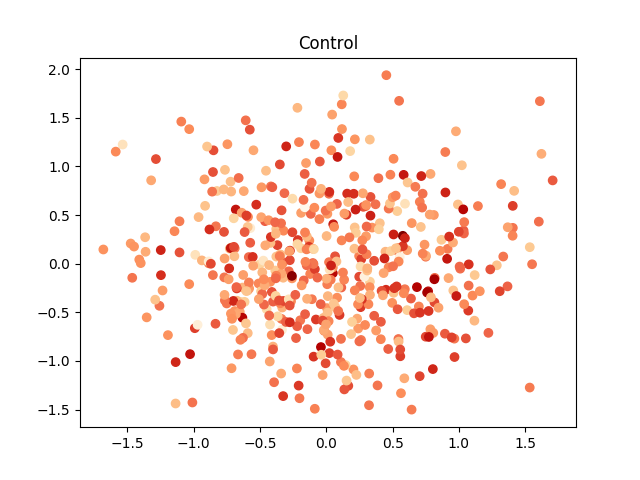
\includegraphics[width=\linewidth]{graphs/Control__pca.png}
    \caption{Initial Population}
  \end{subfigure}
  \begin{subfigure}[b]{0.4\linewidth}
    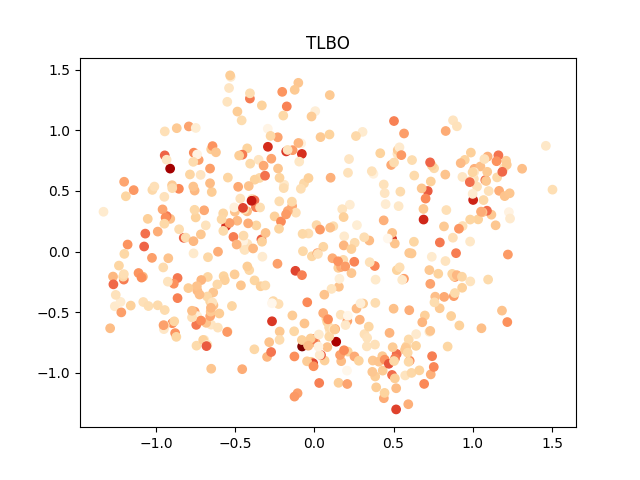
\includegraphics[width=\linewidth]{graphs/TLBO__pca.png}
    \caption{TLBO Population}
  \end{subfigure}
  \caption{Example of Metaheuristic Clustering Behavior}
  \label{fig:coffee}
\end{figure}

\begin{figure}[h!]\label{higherpca}
  \centering
  \begin{subfigure}[!h]{0.4\linewidth}
    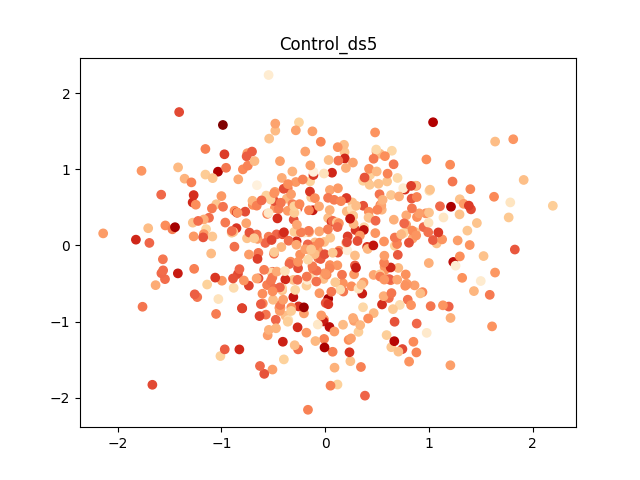
\includegraphics[width=\linewidth]{graphs/Control_ds5__pca.png}
    \caption{Initial Population}
  \end{subfigure}
  \begin{subfigure}[!h]{0.4\linewidth}
    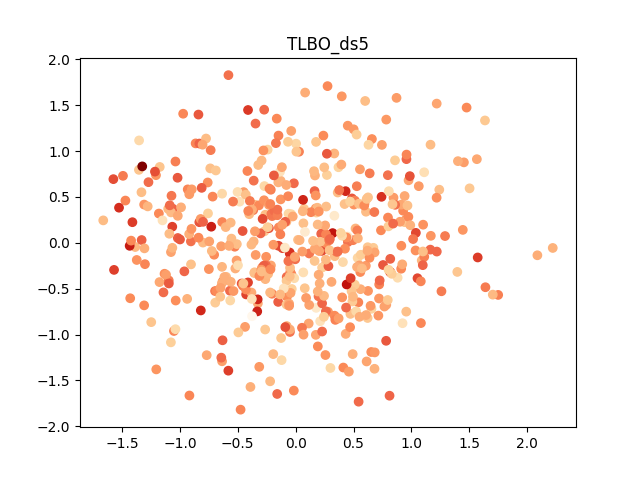
\includegraphics[width=\linewidth]{graphs/TLBO_ds5__pca.png}
    \caption{TLBO Population}
  \end{subfigure}
  \caption{Clustering Behavior on a Higher Dataset}
  \label{fig:coffee}
\end{figure}

Figure \ref{higherpca} shows that the clustering effect is less visible on a higher dataset with more variables. To determine if this is due to the clustering being less prevalent on problems with more variables, or PCA being a less effective visualization, it is necessary to create a metric to measure diversity. 

The diversity metric is defined at Algorithm \ref{divmet}. 



\begin{algorithm}
\caption{Diversity Metric}
\label{divmet}
\begin{algorithmic}
\STATE total = 0
\FOR{solution $\in$ population}
\STATE distances = [euclidean\_distance(solution, sol2) for sol2 in population]
\STATE sort(distances)
\STATE total += sum(distances[1:4])
\ENDFOR
\RETURN total$\div$(length(population)*3)
\end{algorithmic}
\end{algorithm}

\clearpage
The average diversity metrics for the results for the Beasley MDMKP dataset are shown in Table \ref{solodiv}. 


\begin{table}[htbp]
  \resizebox{0.8\textwidth}{!}{\begin{minipage}{\textwidth}
        \caption{Metaheuristic Diversity Results}
        \csvautotabular{data/rounded_solo_diversity.csv}\label{solodiv}
      \end{minipage}}
\end{table}

We see that all the metaheuristics tested (except Local Flip, a subset of VND) are intensification techniques. As population-based metaheuristics rely on creating new solutions from diverse inspiration solutions, a loss of diversity will lead to a loss of effectiveness. It is therefore beneficial to devise a method to limit the progressive diversity loss. 

There are several methods to limit loss of diversity, such as expanding the solution pool, reintroducing old, poorly performing outlier solutions to the population, or ensuring that any new solution replacing an old solution must be suffiently different to every other solution in the population, which is the strategy used in this implementation. 

To ensure that new solutions are significantly unique, the VND local search is attempted on every solution generated by other metaheuristics. This makes it impossible for two solutions differing in only one bit to be a part of the population, and has the added benefit of reducing the search space from finding the best solution, to finding the best solution watershed. Results for this method are shown in Table \ref{sololsdiv}. We see that generally, methods with local search embedded have a higher diversity than methods without. 


\begin{table}[htbp]
  \resizebox{0.4\textwidth}{!}{\begin{minipage}{\textwidth}
        \caption{Metaheuristic Local Search Diversity Results}
        \csvautotabular{data/rounded_solo_ls_diversity.csv}\label{sololsdiv}
      \end{minipage}}
\end{table}

Combining a local search with other metaheuristics is a strategy that has been tried before, for example by Dr. Vasko et. al. \cite{mmkp}. However, Dr. Vasko et. al. created a hybrid method consisting on a local search followed by some other metaheuristic. Testing has shown that this implementation's method of embedding a local search, rather than prefixing one, reduces the percent deviation from the optimal by five to ten times for some metaheuristics.

When the embedded local search strategy is used, it is also embedded into the initial population generation algoritm, in order to prevent initial solutions adjacent to a local minima from becoming "stuck" in the population. 

\section{Comparing Metaheuristics} \label{compare}

Some metaheuristics, such as LBO and GA, are very similar for some circumstances. It would be advantageous to be able to quantify exactly how similar these algorithms are. This can be done by totalling the Manhattan distances between the linear assigment of one resultant population to another. 

Manhattan distance, also called cityblock distance, is a measure of the discrete steps needed to turn one solution into another. For binary problems, it is a measure of how many bits are different. 

Linear Assignment, or the Assignment Problem, is the process of assigning $n$ agents to $n$ tasks to minimize the cost of assignment\footnote{See https://bit.ly/2wPh9mQ for a visualization}. 

For every problem, an assignment cost can be computed between the resulting populations of two metaheuristics. A cost matrix can be constructed from a set of metaheuristics. Averaging the cost matrixes for every problem in a dataset will increase consistency of the results. 

The size of this matrix increases quadratically to the amount of metaheuristics tested. It quickly becomes incomprehensible to look at even a small matrix:	

\begin{table}[htbp]
  \resizebox{0.2 \textwidth}{!}{\begin{minipage}{\textwidth}
        \caption{Distance Matrix}
        \csvautotabular{data/rounded_ds5_matrix_limited.csv}
      \end{minipage}}
\end{table}

An algorithm called Multi-Dimensional Scaling will attempt to find a low dimensional mapping of a cost matrix such that the sum of the squares of the differences of the distances between points among the high and low dimensional space is minimized. The MDS graph is much more comprehensible:

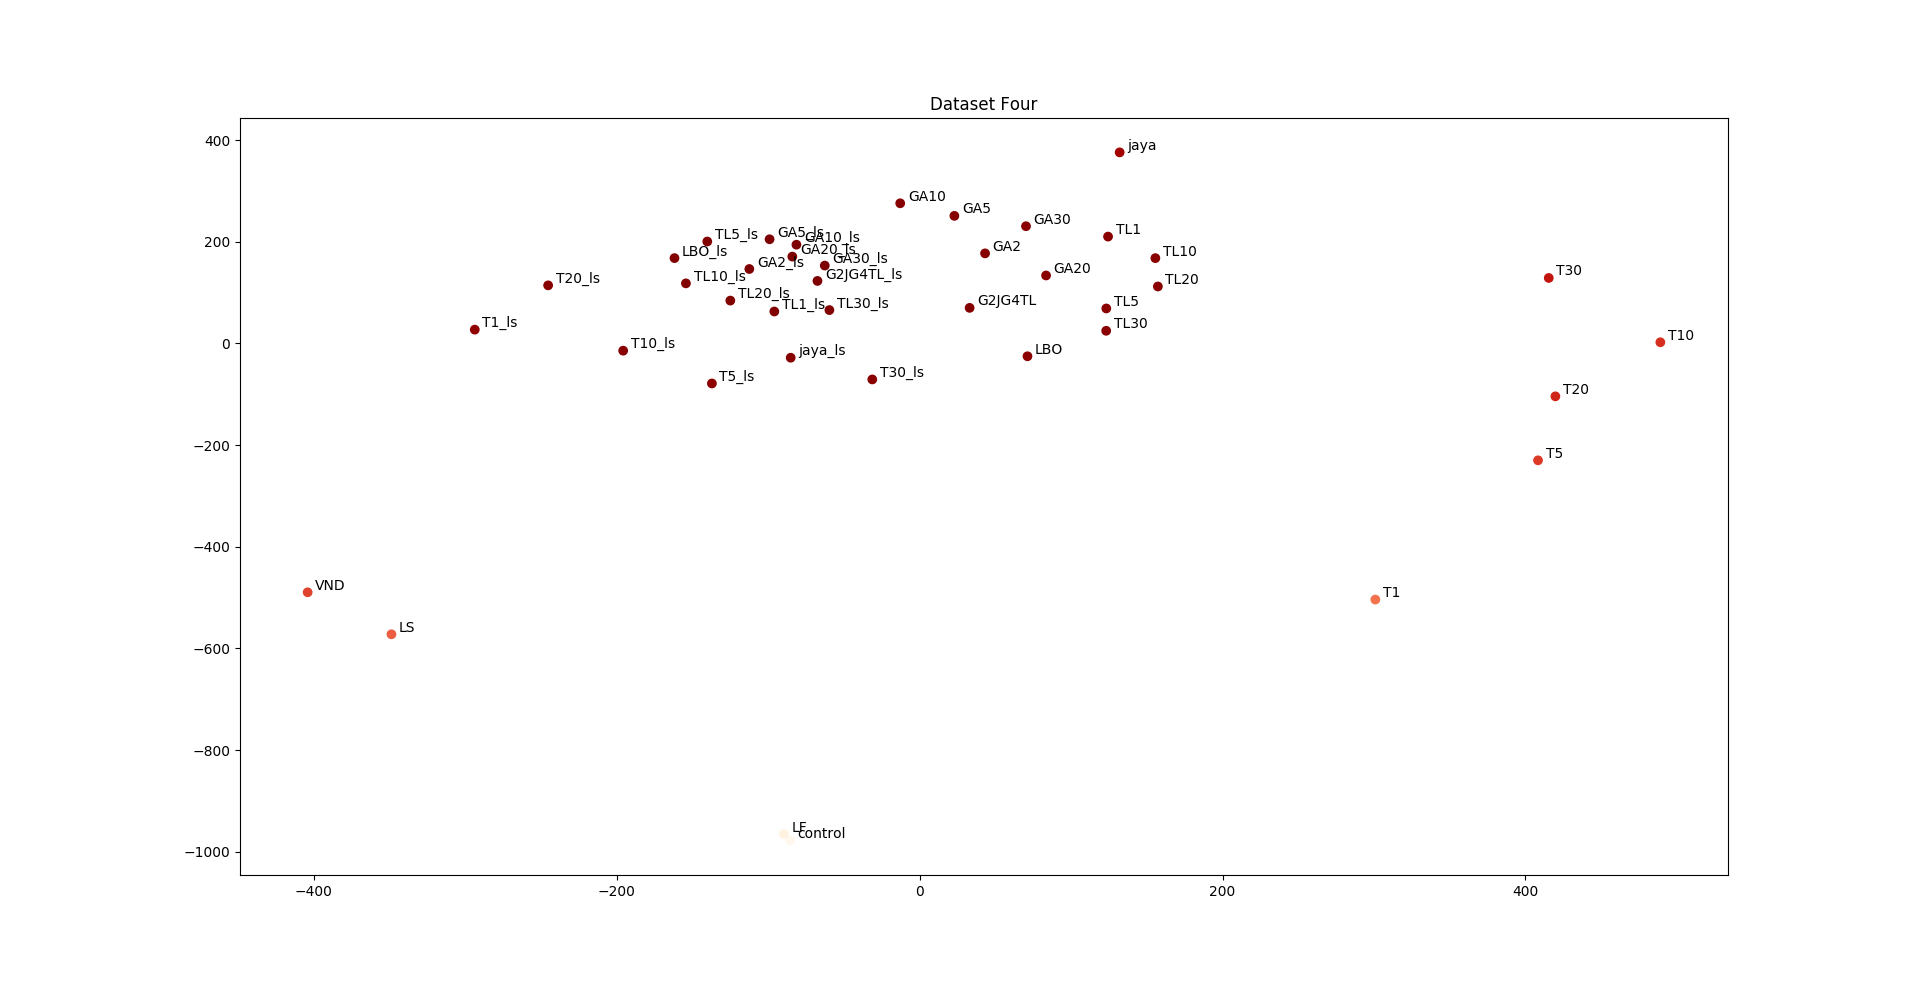
\includegraphics[width=\linewidth]{graphs/ds4_matrix.png}

This is the graph for only dataset four, as generating the cost matrix is quite computationally expensive. 

The darkness of the color signifies the relative performance of the best scoring solution: 100\% dark signifies the metaheuristic had the best performing solution, and 0\% dark is the worst performing. The other colors are scaled linearly.  

\section{Choosing Parameters}

A large search of many different parameter combinations, as has been done to calculate diversities and the MDS graph, requires testing of nearly 80 different metaheuristic instances. Practical reasons therefore limit the amount of time each metaheuristic is allowed to take---so far, each algorithm has been given 4 seconds of run time. A 60 second time limit will more accurately match practical applications of these techniques. Therefore, it is necessary to choose a subset of promising metaheuristics to test. 

Metaheuristics worth testing will satisfy at least one of two criteria: they will give competetive results, or they will have unique behavior. The MDS graph will show metaheuristics with unique behavior, and a complete search of a few datasets will give an indication of performance. See Table \ref{ds4percent}.

\begin{table}[htbp]
  \resizebox{0.4 \textwidth}{!}{\begin{minipage}{\textwidth}
        \caption{Fast Large Percentage Search}
        \csvautotabular{data/rounded_ds4_percentages.csv}\label{ds4percent}
      \end{minipage}}
\end{table}

We see that the Genetic Algorithm beats out every other metaheuristic, regardless of its parameters. It is followed by TLBO and LBO. Unweighted LBO should be very similar to the Genetic Algorithm with two parents, the only difference lies in how parents are selected from the population, so it is surprising to see it this low in the list. Next lies Jaya and TBO with high values for $m$ and $n$. CBO is very poorly performing, and joins the bottom of the list with low valued Jaya and TBO, as well as local search methods with no accompanying global method. 

Since the Genetic Algorithm has similar behavior no matter the amount of parents, only one instance needs to be tested. Since 2 parents should be similar to LBO given more time, 5 parents will be tested. A local search will be embedded, as it makes a small difference in behavior shown by the MDS graph, but strictly improves performance, as shown by the table. 

TLBO was only tested with a one teacher TBO. Higher teacher values improve performance of TBO, but this may not be true for TLBO. Therefore, TLBO will be tested with one, 15,and 30 teachers for TBO. The MDS graph shows that TLBO will have a similar behavior regardless of local search or weighted/unweighted perturbations. Looking to the performance table shows that unweighted with local search performs slightly better than any other instance, so those are the parameters that will be used for further testing. 

Jaya is a metaheuristic that does show a large variation in behavior depending on parameters. The best performing instance has 30 parents, embedded local search, unweighted perturbation, and the most unique instance that is still performant has 3 parents, weighted perturbation, and no local search. Both these instances will be tested. 

CBO behaves very different than any other metaheuristic, as shown by the graph. However, the performance is quite bad, so only one instance needs to be tested. CBO with 30 parents, local search, and a weighted perturbation is the top of the table, so those parameters will be further tested. 

Local searches without an accompanying global method would not benefit from more search time, as they can run to completion within four seconds. 


\subsection{Additional Runtime Parameters}

\paragraph{Maximum Failed Attempts}

When testing a metaheuristic, a single run through is often not enough to extract the full benefits of the method. Instead, it is ran repeatedly, until it fails to produce an improvement for any solution in the population $max\_failed\_attempts$ times in a row. This setting will directly impact the run time of the algorithm. For this longer test, a high value of 25 is used.

\paragraph{Time Constraint}

Each metaheuristic will be given a minute to run. This is a realistic simulation of what would be found in industry. Additionally, some metaheuristic instances can take several seconds to run through one iteration, so a small time value can allot significantly more time to one metaheuristic than another. This effect is mitigated with more time. 


\paragraph{Population Size}

The population generation procedure will be ran until 30 solutions are generated, or 500,00 attempts are made. If less than 30 solutions are found, which can happen for some datasets, metaheuristic optimization is attempted anyway. Local search is embedded into the initial population generation.

\section{Results}

Below are tables showing the percent deviation from optimal for each algorithm. Each algorithm had the same initial population, generated using an embedded local search. "Control" is therefore equivalent to the VND metaheuristic. 

Optimal values were calculated using a CPLEX program given two hours to search for the best solution. For datasets 5, 7, 8, and 9, the metaheuristics found solutions better than the CPLEX reported optimals. These negative percentages result in a misleadingly low optimal. 

Additionally, dataset 7 has many problems that are extremely difficult to find feasible solutions for. Therefore, 7 is more of a test of the initial population generation algorithm than any specific metaheuristic. If the initial population generator finds a solution CPLEX did not, it is reported as 0\% error, but if the inverse happens, it is 100\% error. This leads to a deceptively high average. 

Averaging only datasets 1, 2, 3, 4 and 6 from the hybrid method with embedded local search gives an overall lowest percentage of 0.27\%. 

\begin{table}[htbp]
  \resizebox{0.6\textwidth}{!}{\begin{minipage}{\textwidth}
        \caption{Metaheuristic 10 Second Results}
        \csvautotabular{data/rounded_solo_10s_percentages.csv}
      \end{minipage}}
\end{table}

\begin{table}[htbp]
  \resizebox{0.6\textwidth}{!}{\begin{minipage}{\textwidth}
        \caption{Metaheuristic 60 Second Results}
        \csvautotabular{data/rounded_solo_60s_percentages.csv}
      \end{minipage}}
\end{table}


\begin{table}[htbp] 
  \resizebox{0.6\textwidth}{!}{\begin{minipage}{\textwidth}
        \caption{Hybrid 60 Second Results}
        \csvautotabular{data/rounded_hybrid_60s_percentages.csv}
      \end{minipage}}
\end{table}


\section{Creating a Hybrid Method}

A hybrid method consisting of many metaheurisitcs chained together has the potential to outperform any one metaheuristic, but the order of metaheuristics must be chosen with care. Putting a strongly intensifying metaheuristic too early in the chain can cripple the population for the next metaheuristic. This can be somewhat mitigated by running each metaheuristic only once before looping through the chain, as opposed to running one technique to exhaustion before moving on to the next. However, the order can still have a significant effect. 

Using the table of diversities, as well as the general principle that intensification and diversification should oscillate, and the goal of including each metaheuristic only once, the patterns TLJB, TBJL, JBTL, and TLJB result. Keeping TBO and LBO consecutive due to the effectiveness of the TLBO method, and including the GA twice, once with two parents, once with four parents, gives the chain GA[parents=2], Jaya, GA[parents=4], TBO, LBO. 

\subsection{Additional Visualizations}

\begin{figure}[h!]
  \centering
  \begin{subfigure}[b]{0.4\linewidth}
    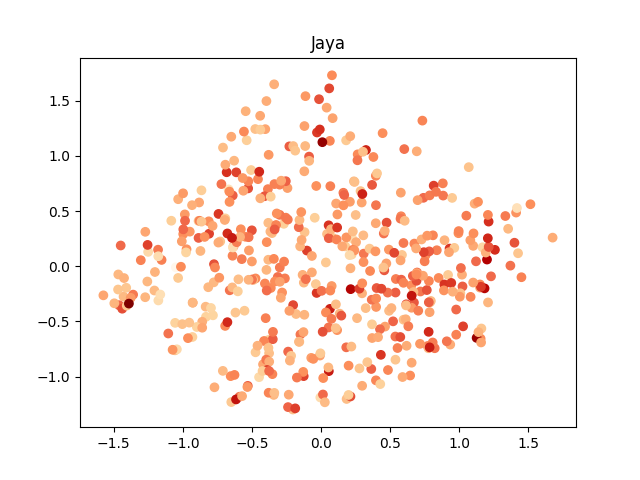
\includegraphics[width=\linewidth]{graphs/Jaya__pca.png}
  \end{subfigure}
  \begin{subfigure}[b]{0.4\linewidth}
    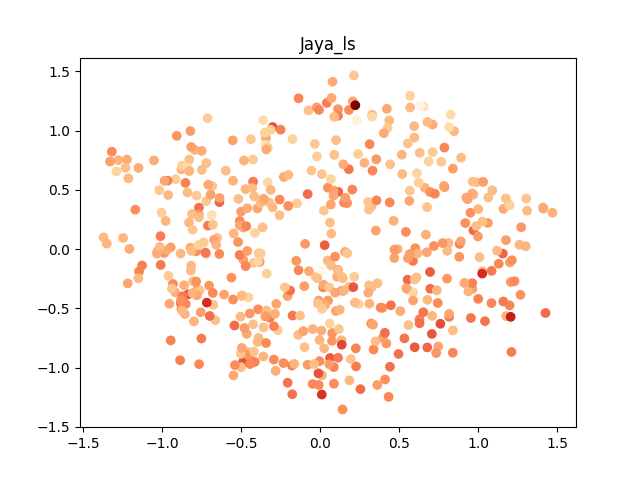
\includegraphics[width=\linewidth]{graphs/Jaya_ls__pca.png}
  \end{subfigure}
  \caption{Jaya and Jaya Local Search}
  \label{fig:coffee}
\end{figure}

\begin{figure}[h!]
  \centering
  \begin{subfigure}[b]{0.4\linewidth}
    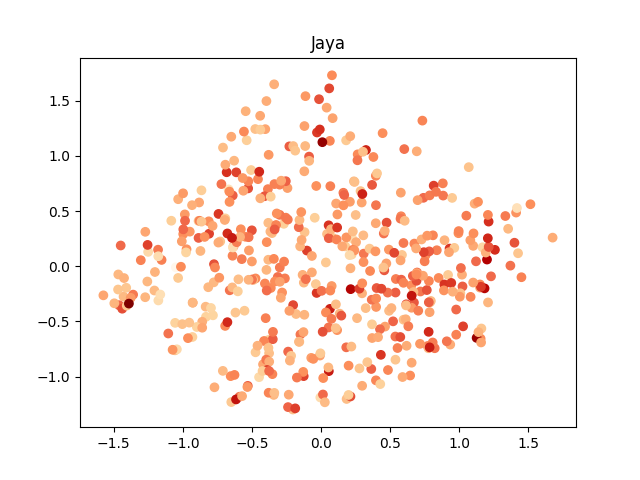
\includegraphics[width=\linewidth]{graphs/Jaya__pca.png}
  \end{subfigure}
  \begin{subfigure}[b]{0.4\linewidth}
    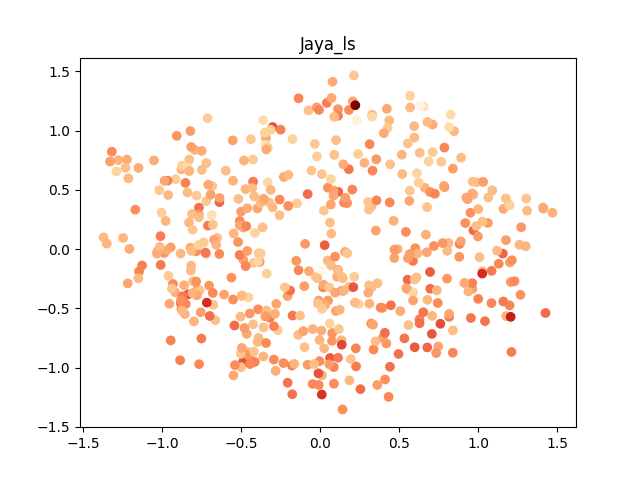
\includegraphics[width=\linewidth]{graphs/Jaya_ls__pca.png}
  \end{subfigure}
  \caption{Jaya and Jaya Local Search}
  \label{fig:coffee}
\end{figure}

\begin{figure}[h!]
  \centering
  \begin{subfigure}[b]{0.4\linewidth}
    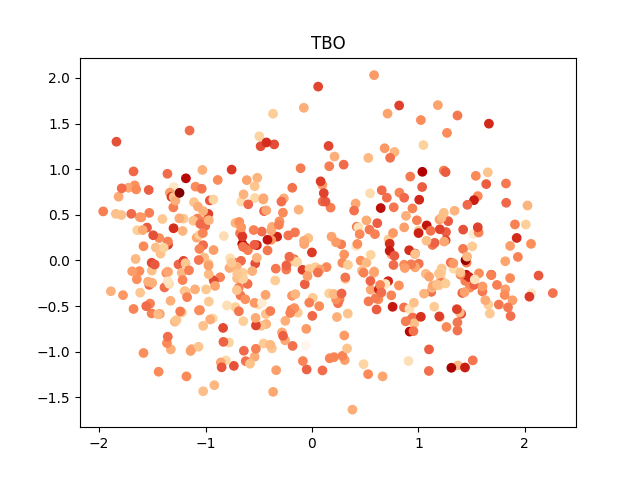
\includegraphics[width=\linewidth]{graphs/TBO__pca.png}
  \end{subfigure}
  \begin{subfigure}[b]{0.4\linewidth}
    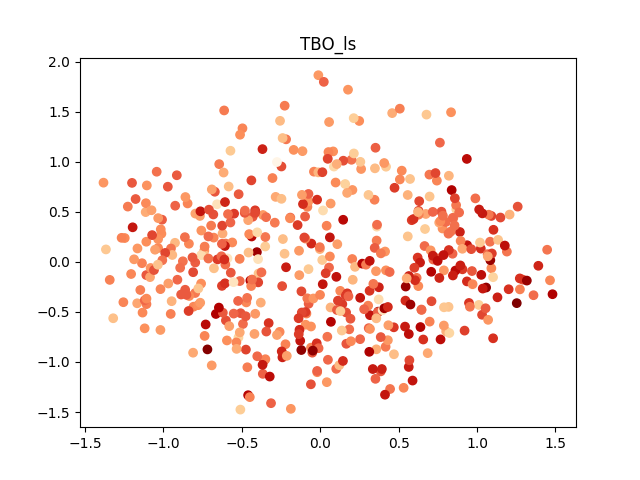
\includegraphics[width=\linewidth]{graphs/TBO_ls__pca.png}
  \end{subfigure}
  \caption{TBO and TBO Local Search}
  \label{fig:coffee}
\end{figure}

\begin{figure}[h!]
  \centering
  \begin{subfigure}[b]{0.4\linewidth}
    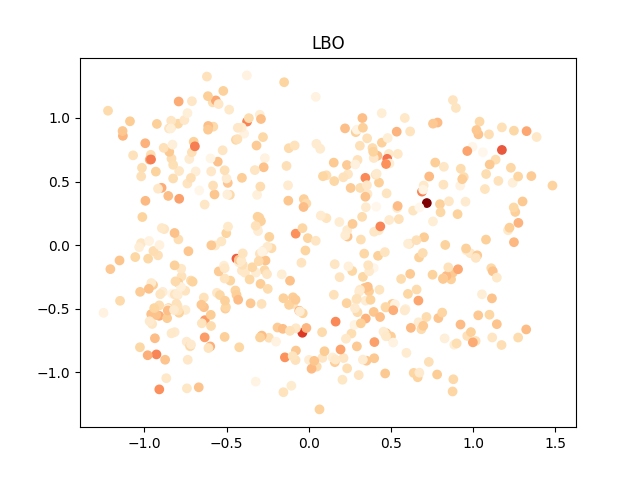
\includegraphics[width=\linewidth]{graphs/LBO__pca.png}
  \end{subfigure}
  \begin{subfigure}[b]{0.4\linewidth}
    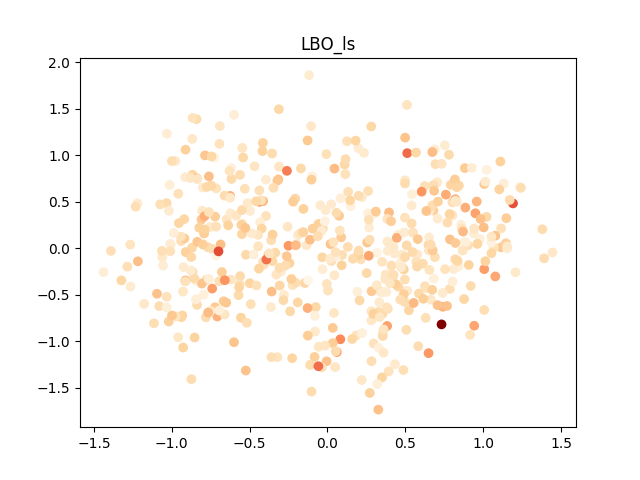
\includegraphics[width=\linewidth]{graphs/LBO_ls__pca.png}
  \end{subfigure}
  \caption{LBO and LBO Local Search}
  \label{fig:coffee}
\end{figure}

\begin{figure}[h!]
  \centering
  \begin{subfigure}[b]{0.4\linewidth}
    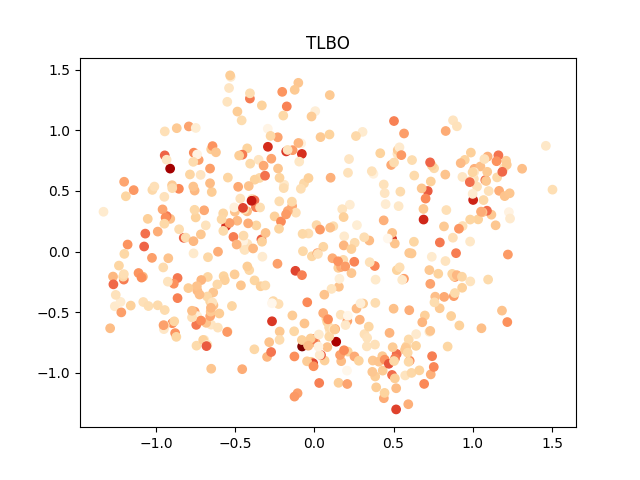
\includegraphics[width=\linewidth]{graphs/TLBO__pca.png}
  \end{subfigure}
  \begin{subfigure}[b]{0.4\linewidth}
    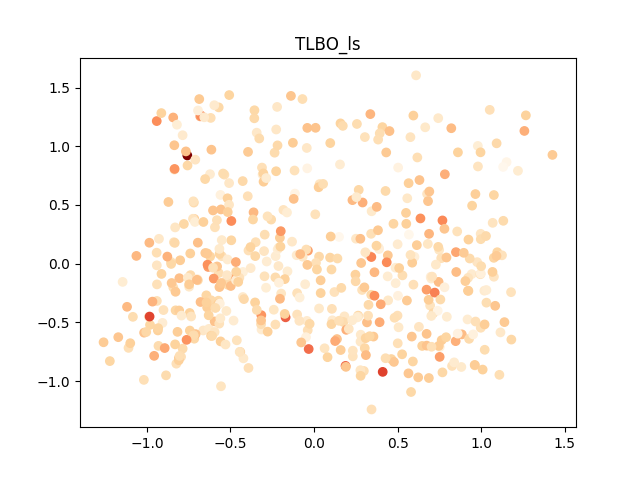
\includegraphics[width=\linewidth]{graphs/TLBO_ls__pca.png}
  \end{subfigure}
  \caption{TLBO and TLBO Local Search}
  \label{fig:coffee}
\end{figure}

\begin{figure}[h!]
  \centering
  \begin{subfigure}[b]{0.4\linewidth}
    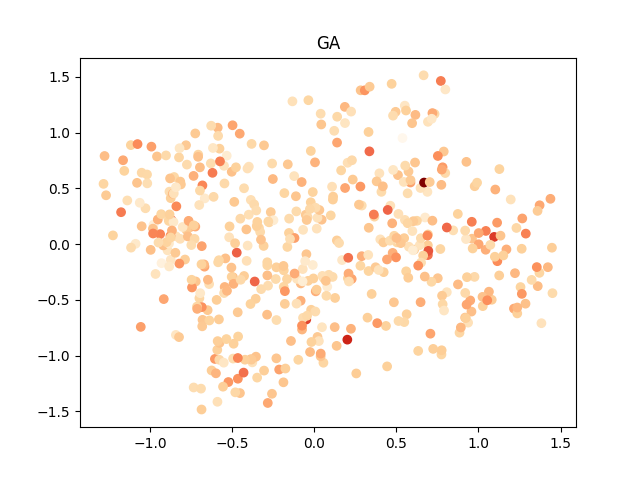
\includegraphics[width=\linewidth]{graphs/GA__pca.png}
  \end{subfigure}
  \begin{subfigure}[b]{0.4\linewidth}
    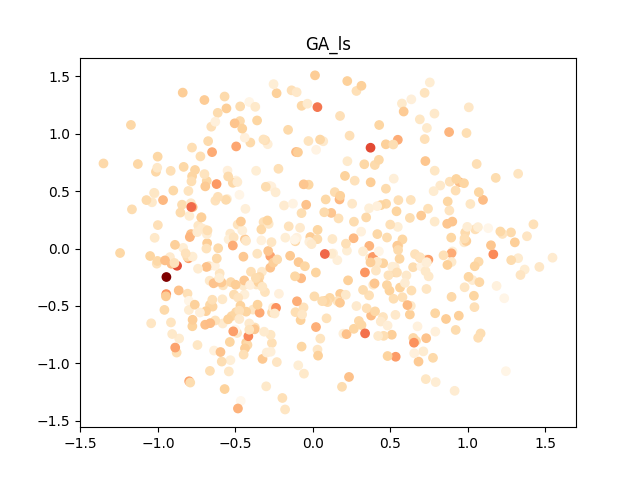
\includegraphics[width=\linewidth]{graphs/GA_ls__pca.png}
  \end{subfigure}
  \caption{GA and GA Local Search}
  \label{fig:coffee}
\end{figure}

\begin{figure}[h!]
  \centering
  \begin{subfigure}[b]{0.4\linewidth}
    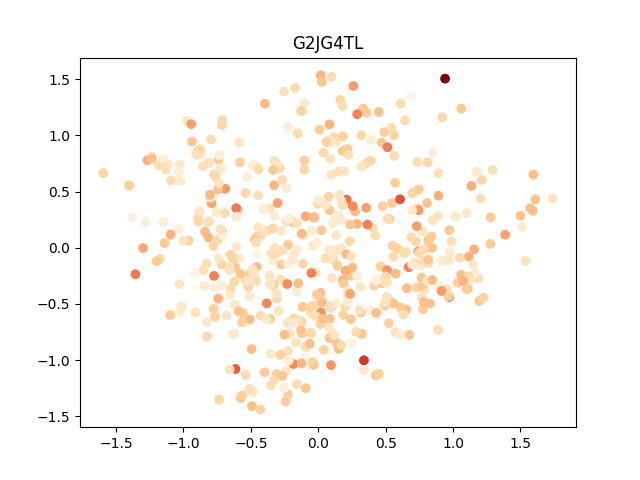
\includegraphics[width=\linewidth]{graphs/G2JG4TL__pca.png}
  \end{subfigure}
  \begin{subfigure}[b]{0.4\linewidth}
    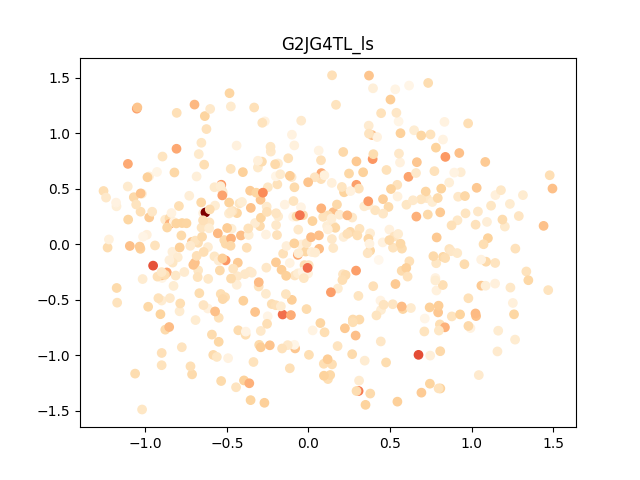
\includegraphics[width=\linewidth]{graphs/G2JG4TL_ls__pca.png}
  \end{subfigure}
  \caption{G2JG4TL and G2JG4TL Local Search}
  \label{fig:coffee}
\end{figure}

\clearpage 


\bibliography{methods}
\bibliographystyle{plain}
\end{document}
